
\subsection{相似性保留加密}
\label{subsec:featurespy-spe}

本文提出了相似性保留加密(similarity-preserving
encryption, SPE),它同时建立在消息锁加密密钥和基于特征的加密之上,通过消息锁加密密钥减轻密钥泄露导致的安全威胁,同时通过基于特征的加密密文数据块相似性。具体来说(如图~\ref{fig:featurespy-design-spe}所示),由于相似数据块的内容差异有限,相似性保留加密从每个明文数据块中抽取一小部分(例如,前32个字节,占8\,KiB数据块的0.4\%),称为相似性指标({\tt similarity indicator}),由此产生的相似数据块的相似性指标很可能是相同的。相似性保留加密使用基于特征的加密方案加密相似性指标,而剩余的大部分(占 8\,KiB数据块的99.6\%)数据块内容用消息锁加密。基于此,\sysnameF 可以通过检验密文数据块的相似性指标(例如,每个密文数据块的前32个字节)是否相同来检测密文数据块的相似性。由于相同的数据块共享相同的内容特征(产生相同的特征密钥)和消息锁加密密钥,消息保留加密不会降低跨用户加密后重复数据删除(\S\ref{sec:background-enc-deduplication})的存储效率。

\begin{figure}[!htb]
    \centering
    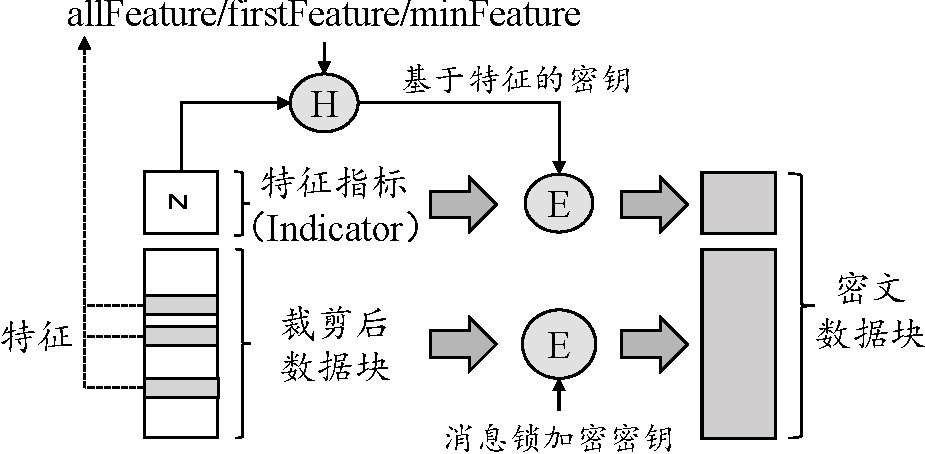
\includegraphics[width=0.7\textwidth]{pic/featurespy/spe.pdf}
    \caption{相似性保留加密方法}
    \label{fig:featurespy-design-spe}
\end{figure}

本文认为消息保留加密减轻了基于特征的加密在密钥泄露时产生的信息泄露风险。这是由于发生密钥泄露的数据块$M$对应的特征密钥只能用于解密与$M$相似的数据块的相似性指标。同时,由于相似数据块本身很可能与数据块$M$具有相同的相似性指标,因此相似性保留加密不会造成额外的信息泄露。即使是少部分与$M$相似但相似性指标不同的数据块收到该密钥泄露的影响,相较于基于特征的加密其泄露的信息也大大减少。下文将详细介绍相似性保留加密的设计细节。

\paragraph*{特征密钥生成。}
如前文所述,本文通过N-transform(\S\ref{subsec:featurespy-basic})为每个明文数据块提取三个顺序的内容特征,一个基本的密钥生成方法(称为 {\tt allFeature})是连接所有特征,并计算基于连接结果的安全哈希产生特征密钥。但是,{\tt allFeature}无法为许多相似较低的数据块生成相同的特征密钥。具体来说,如果相似数据块的内容差异恰好在产生子特征(\S\ref{subsec:featurespy-basic})的滑动窗口中,则数据块将产生不同的特征密钥,使得即使相似性指标原始内容完全相同也无法检查密文数据块的相似性。

本文基于采样的方法\cite{bhagwat2009extreme, dong2011Tradeoffs, qin17}来放宽密钥生成标准。本文为每个明文数据块的所有特征选择以一个代表特征,并根据代表特征计算特征密钥。这样可以容忍相似数据块间更大的内容差异,使得相似度较低的数据块也可产生相同的特征密钥

本文考虑了两种选择代表性特征的方法。具体来说,{\tt firstFeature}根据每个明文数据块的第一个({\tt first})特征生成特征密钥。优点是不需要计算后续的子特征和特征(\S\ref{subsec:featurespy-basic}),减轻N-transform的计算开销 \cite{zhang2019Finesse}。

本文还考虑{\tt minFeature},它建立在Broder定理\cite{broder1997resemblance}的基础上,根据每个数据块所有特征中的最小({\tt minimum})特征(即数值最小值)生成特征密钥。具体来说,Broder定理指出,如果两个明文数据块具有许多共同特征(即,相似的概率很高),它们很可能具有相同的最小特征,即:

\begin{eqnarray}
    \label{eq:featurespy-broder}
    \Pr[\min(S_1) = \min(S_2)] = \frac{|S_1 \cap S_2|}{|S_1 \cup S_2|},
\end{eqnarray}

其中$S_i$是明文数据块$M_i$的特征集合,$\min(S_i)$计算集合 $S_i$($i = 1, 2$)中特征的最小值。因此,{\tt minFeature}倾向于为相似度中等的数据块生成相同的特征密钥。在\S\ref{sec:featurespy-evaluation}中,本文将研究相似性保留加密的不同密钥生成方法的权衡。

此外,除了使用特征生成特征密钥外,另一种设计思路是基于第一个或最小的子特征{\tt sub-feature}生成特征密钥。但由于子特征的信息熵较低,本文不选择这种基于子特征的设计。这是由于根据N-transform的原始配置\cite{shilane12},每个子特征只有4个字节,攻击者可枚举所有可能的子特征/密钥(最高 $2^{32}$)。另一方面,在\S\ref{sec:featurespy-implementation}中,本文重新配置N-transform以确保基于特征的密钥空间足够大(例如,$2^{256}$)以对抗暴力破解攻击。